\section{Attention and Transformers}
\subsection{Sequence-to-sequence with RNNs and attention}
\subsubsection{Encoder-decoder RNNs and limitations}
Originally, the transformer architecture was proposed for machine translation, and was later extended to other deep learning domains. To introduce the attention mechanism, let's consider a machine translation setup; we will start by building up on top of the RNN architecture introduced in the previous chapter.

We are given a sentence in English and want to translate it in French. To do so, we use two RNNs, an encoder which will handling the input tokens, and a decoder which will generate the output sentence.
\begin{figure}[H]
    \centering
    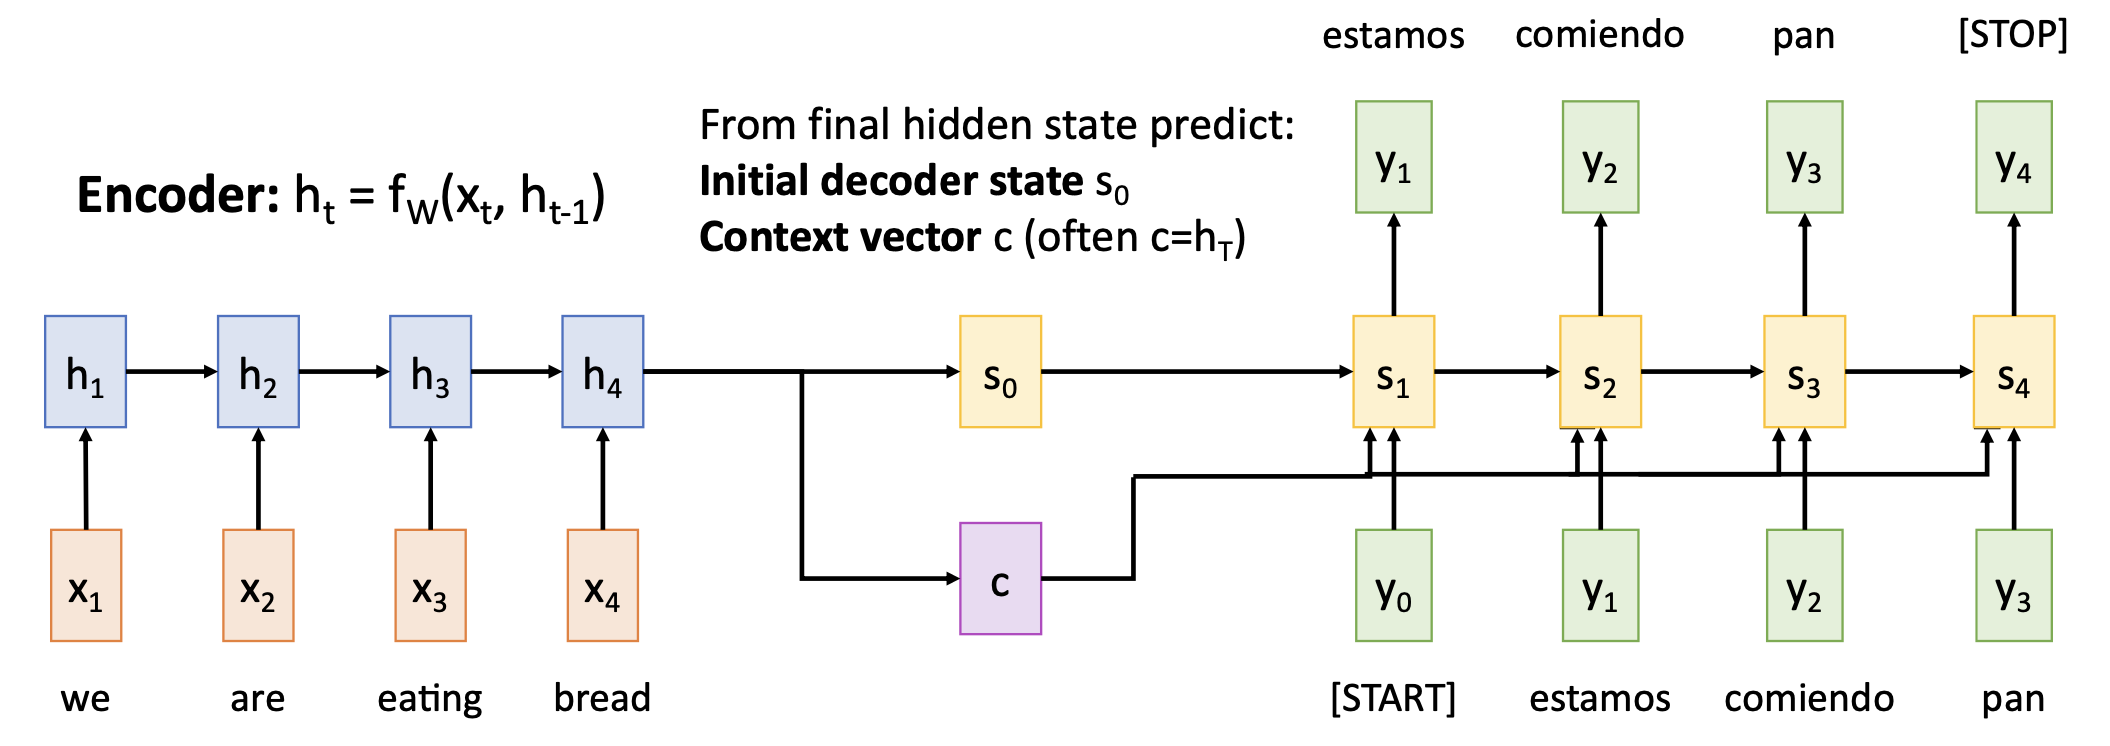
\includegraphics[width=\textwidth]{images/seq-to-seq.png}
    \caption{Sequence-to-sequence using an RNN.}
\end{figure}
After the processing of the original sentence, the encoder will summarize the entire context of that input sentence using two vectors: the initial decoder state $s_0$, and the context vector $c$. In practice, $s_0$ is often obtained by feeding $h_T$ through a feed-forward neural network, and $c$ is often set to $h_T$ directly.

The decoder will receive a start token $y_0$ as its first input, as well as the context vector $c$; it will then generate the first output token $y_1$, which will be used as the second input. Note that the context $c$ is fed to the decoder at each step of the generation, on top of the last generated token $y_t$. Formally, its recurring equation is of the form:
\begin{equation*}
    s_t = g_{W'}(y_{t-1}, s_{t-1}, c)
\end{equation*}

While this architecture is fairly reasonable, its bottleneck is that the entire context of the sentence must be summarized in the fixed-size context vector $c$. If the text to translate is too long (think of an entire book for instance), the model will not be able to fit all the context details in $c$. The idea to solve this issue is to compute a new context vector at each step of the decoder, and to allow the decoder to reconstruct the context vector by using different vectors focusing on different parts of the original sentence. This mechanism is called \emph{attention}.

\subsubsection{The attention mechanism}
We will keep the general encoder-decoder structure, but instead change the way that the context is passed from the encoder to the decoder. We will use an MLP called $f_{\textnormal{att}}$, which will compute scalar alignment scores:
\begin{equation*}
    e_{t,i} = f_{\textnormal{att}}(s_{t-1}, h_i)
\end{equation*}
Intuitively, the alignment score $e_{t,i}\in\R$ quantifies how much \emph{attention} should be put in the hidden state of the encoder $h_i$, given the hidden state of the decoder $s_{t-1}$. These scalars will be used to construct a new context vector at each step of the decoder.

\begin{figure}[H]
    \centering
    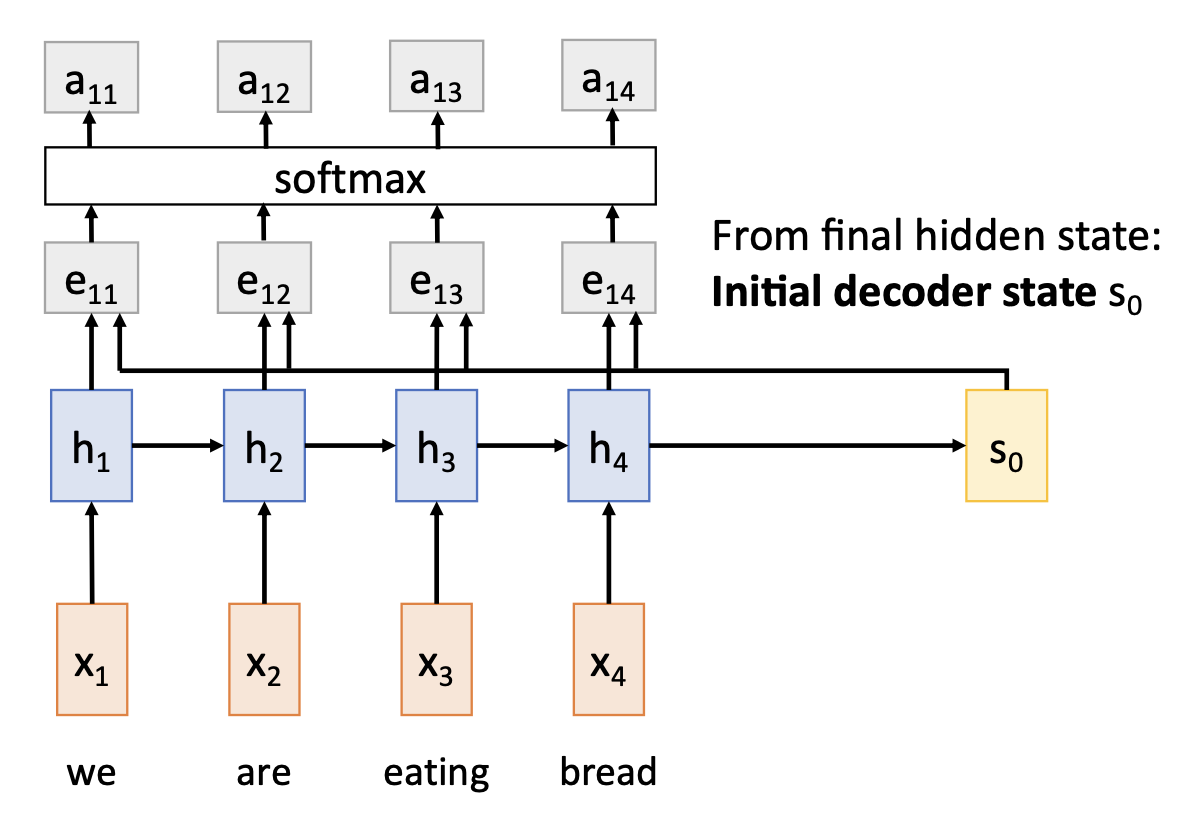
\includegraphics[width=.5\textwidth]{images/attention-scores.png}
    \caption{Applying $\softmax$ to alignment scores gives us attention scores.}
\end{figure}

The alignment scores are arbitrary real numbers. Therefore, we apply to them the $\softmax$ operations for each decoder state $s_{t-1}$, giving us \emph{attention weights} $(a_{t,i})$ satisfying:
\begin{equation*}
    \sum_i a_{t,i} = 1 
\end{equation*}
That being done, we can finally compute the context vector for each time step $t$ of the decoder, using a sum of the hidden states $(h_i)$ weighted by the attention scores $(a_{t,i})$:
\begin{equation*}
    c_t = \sum_i a_{t,i} h_i
\end{equation*}
This gives us the context vector $c_t$ which will be used for the generation of $y_t$ by the decoder. Note that this is all differentiable and allows us to backpropagate through the parameters of $f_{\textnormal{att}}$; in particular, we do not need to supervise the attention weights.
\begin{figure}[H]
    \centering
    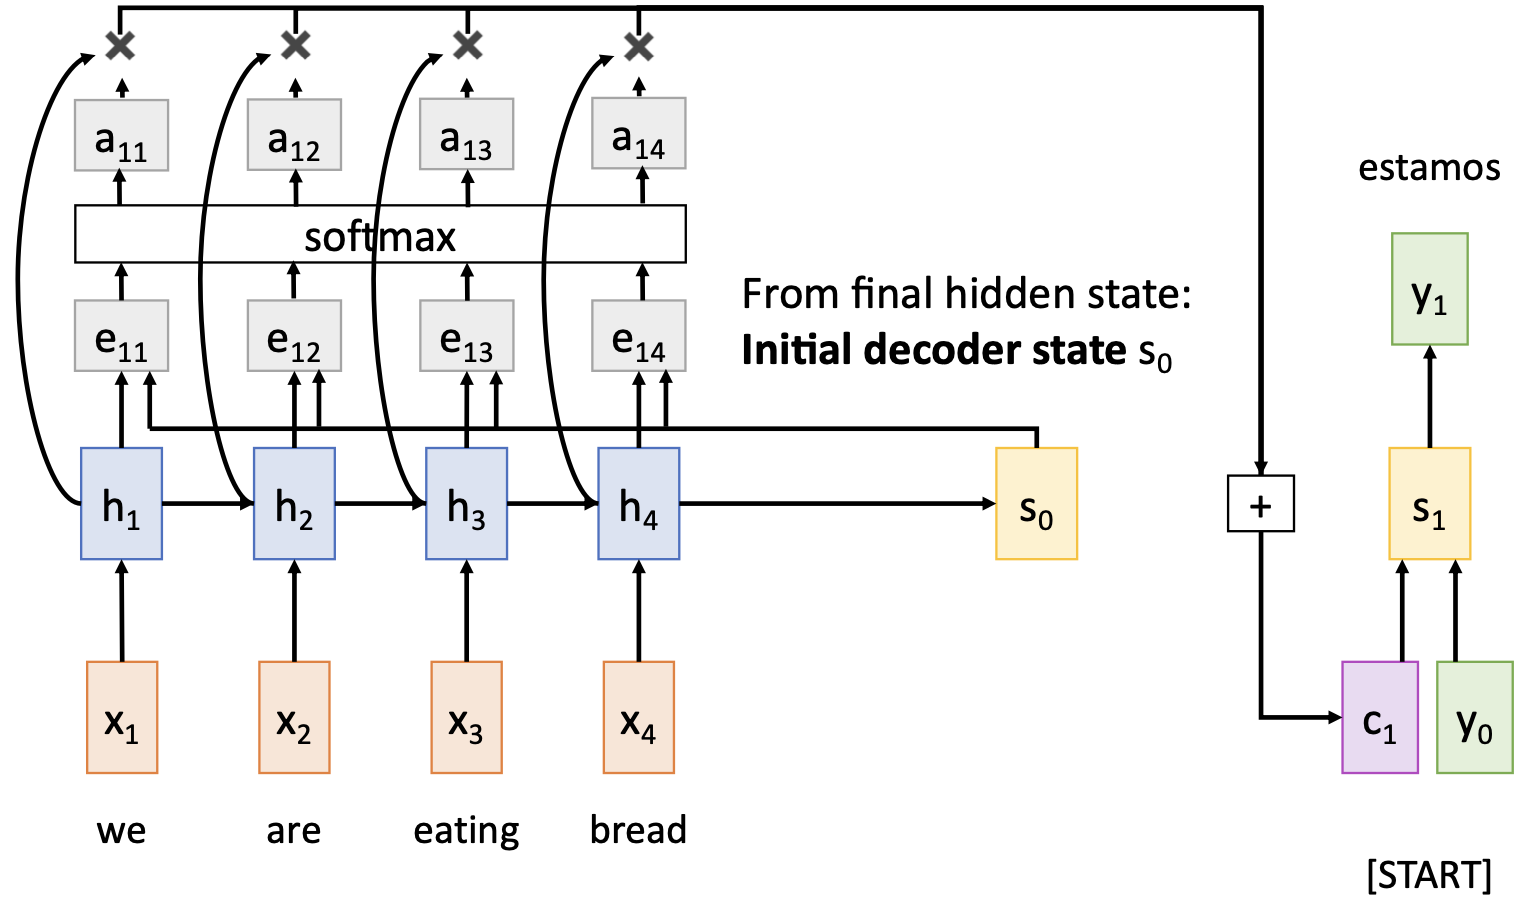
\includegraphics[width=.65\textwidth]{images/attention-context.png}
    \caption{Computation of the context vector using attention scores.}
\end{figure}
This process that was applied for the first decoder step $t=1$ can be iterated for every following step: we compute the alignment scores using the new hidden state $s_1$, then the attention scores, giving us the context vector $c_t$, which is fed into the decoder alongside $y_{t-1}$.
\begin{figure}[H]
    \centering
    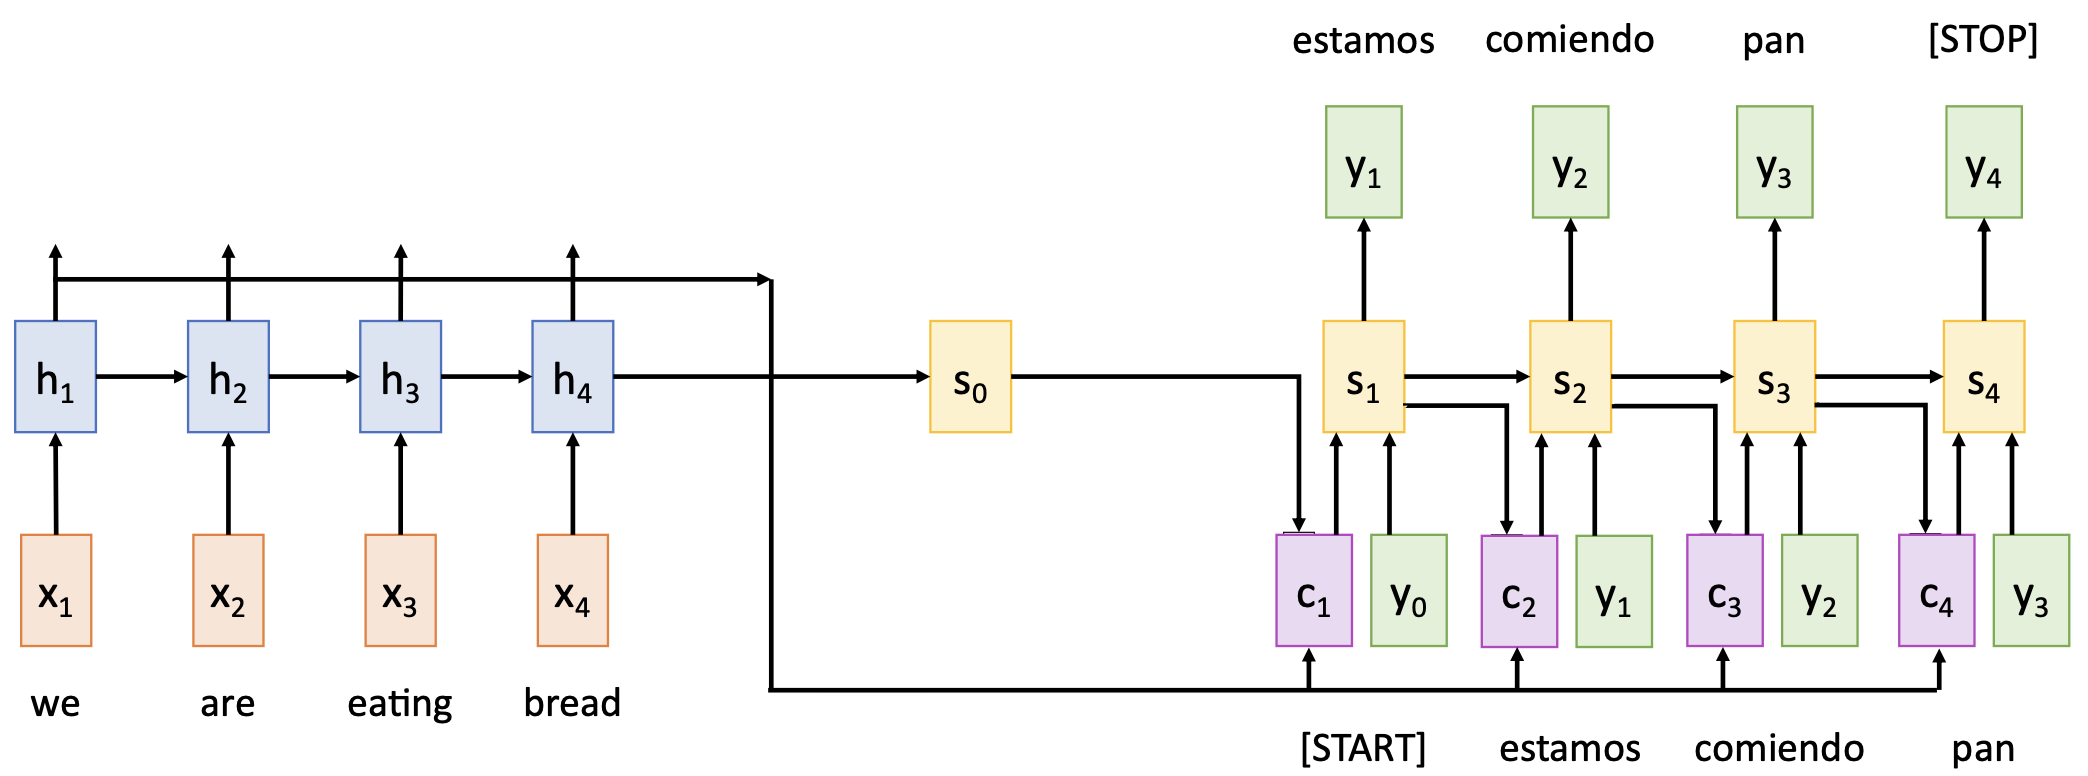
\includegraphics[width=.9\textwidth]{images/attention-unrolled.png}
    \caption{Unrolling the computational graph with attention.}
\end{figure}
This overcomes the bottleneck problem encountered for unique context vectors: at each step, the decoder is able to choose the relevant hidden states of the encoder, which selects only relevant information. When working with very long sequences, the model will be able to shift its attention around and focus on important parts of the inputs.

\subsection{Visualizing and interpreting attention weights}
\begin{wrapfigure}[14]{r}{.45\textwidth}
    \captionsetup{justification=raggedleft}
    \centering
    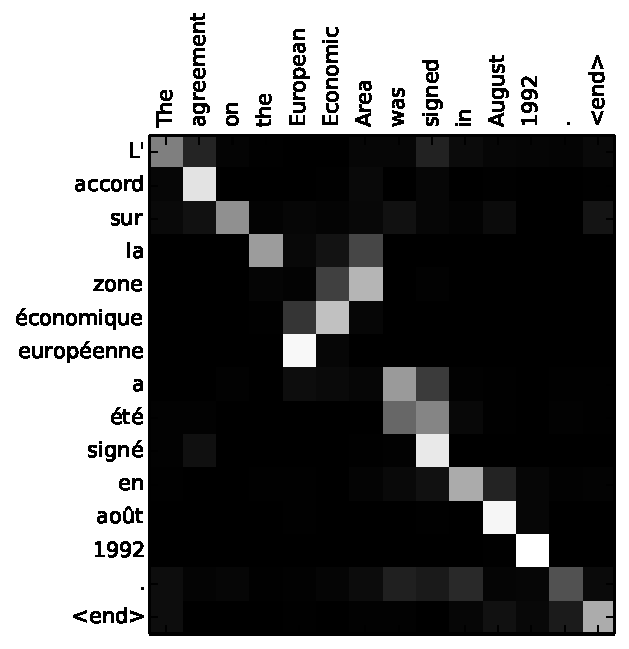
\includegraphics[width=.45\textwidth]{images/attention-visualization.pdf}
    \caption{Visualization of attention weights for English-to-French translation.\protect\footnotemark}
\end{wrapfigure}
\footnotetext{Image taken from Bahdanau et al., \say{Neural machine translation by jointly learning to align and translate}, ICLR 2015}
The attention weights can be used to gain interpretability of the model: we can see for each output word which original words it was the most focused on.  

Diagonal attention (the first four words and the last 5 words) means that words correspond in order between French and English. High coefficients outside the diagonal (for instance, \say{European}/\say{européenne}) show words out of order between the two sentences. Finally, some lines and columns have more than one non-zero coefficient, such as the \say{was} or \say{say} columns: these show that the verb conjugation requires more than one word of context to be translated.

\newpage
\subsection{Image captioning with RNNs and Attention}
It is important to notice that the decoder does not use the fact that the hidden states $(h_i)_i$ form an ordered sequence, but only considers them as an unordered set $\set{h_i}{i\in I}$. This means that we can use the same architecture given any set of input hidden vectors $\set{h_i}{i\in I}$, especially for other types of data that do not form sequences.

Consider a deep convolutional neural network, without fully-connected layers at the end. The ouput of this CNN can be interpreted as a grid of feature vectors of the image. We see these feature vectors just like a sequence of hidden states of an encoder RNN: we can therefore apply the attention mechanism to them. We consider a simple model $f_{\textnormal{acc}}$ that we use to compute the alignment scores of each feature in the grid:
\begin{equation*}
    e_{t,i,j} = f_{\textnormal{att}}(s_{t-1}, h_{i,j})
\end{equation*}
We then pass each grid of alignment scores into the $\softmax$ operator, giving us a normalized probability distribution, the grid of attention weights $(a_{t,i,j})$. Once again, the context of the image can be summarized with respect to the attention weights by computing a context vector $c_t$:
\begin{equation*}
    c_t = \sum_{i,j} a_{t,i,j} h_{i,j}
\end{equation*} 
Feeding the context vector $c_1$ alongside the start token $y_0$ into the decoder RNN starting with hidden state $s_0$ can be used to generate a caption corresponding to the image.
\begin{figure}[H]
    \centering
    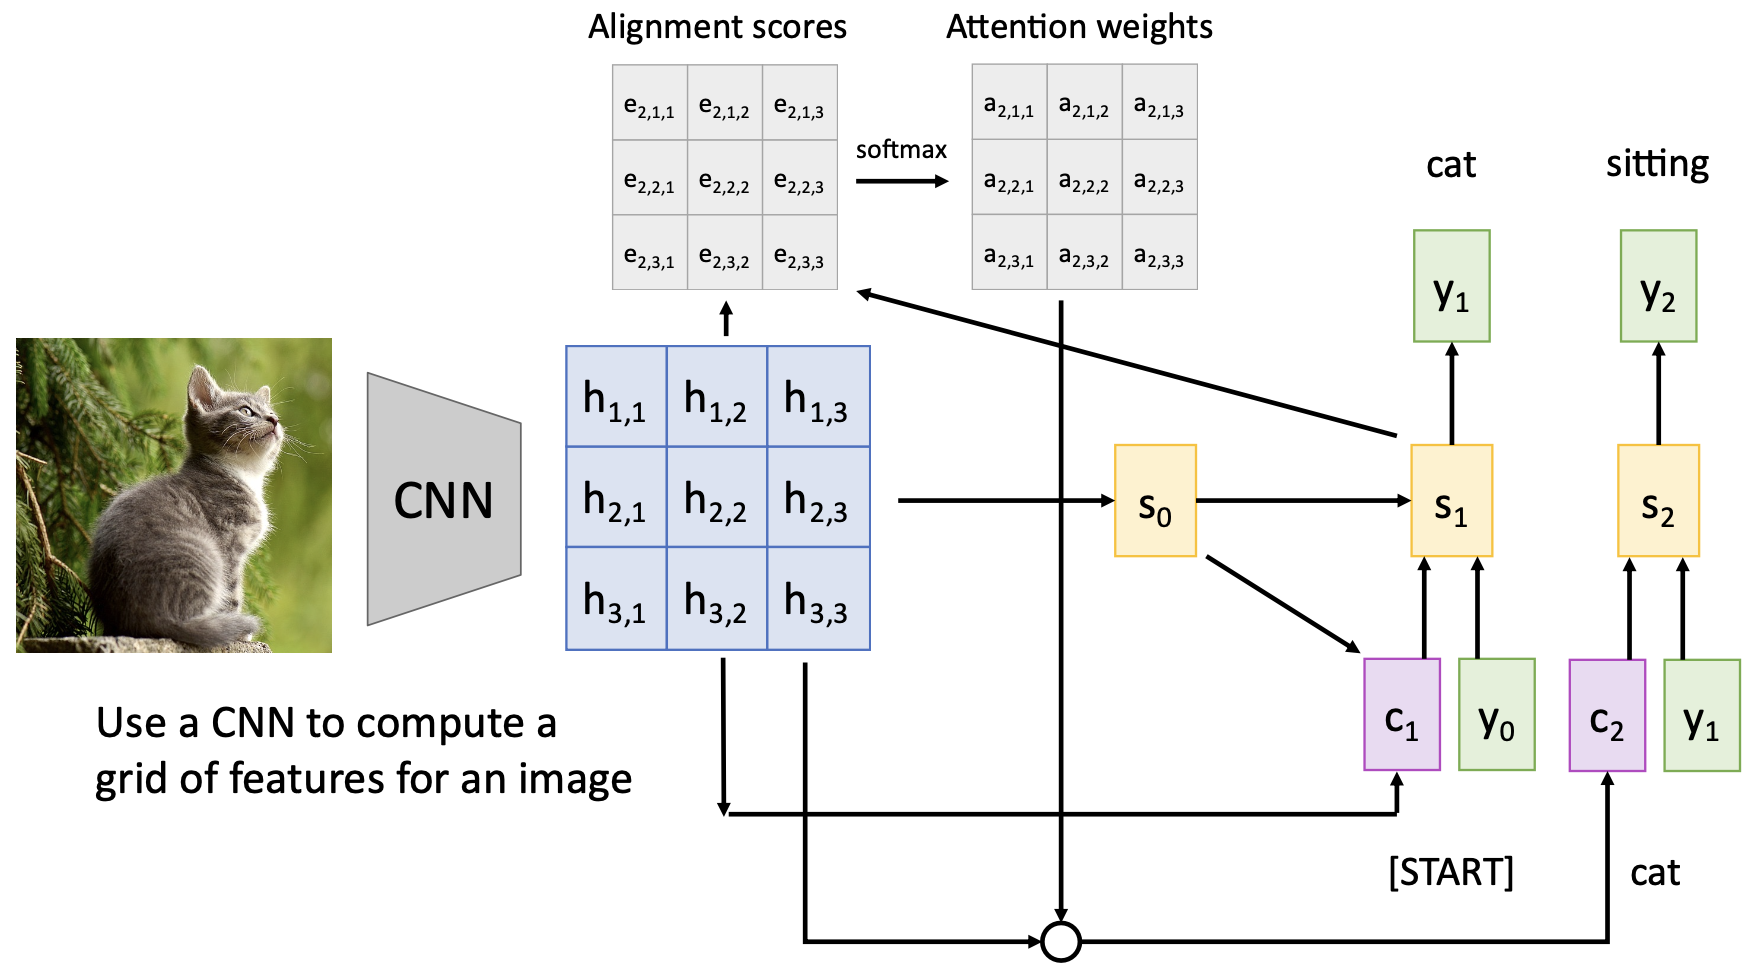
\includegraphics[width=.9\textwidth]{images/attention-cnn.png}
    \caption{Applying attention to a grid of features for image captioning.}
\end{figure}

\begin{figure}[H]
    \centering
    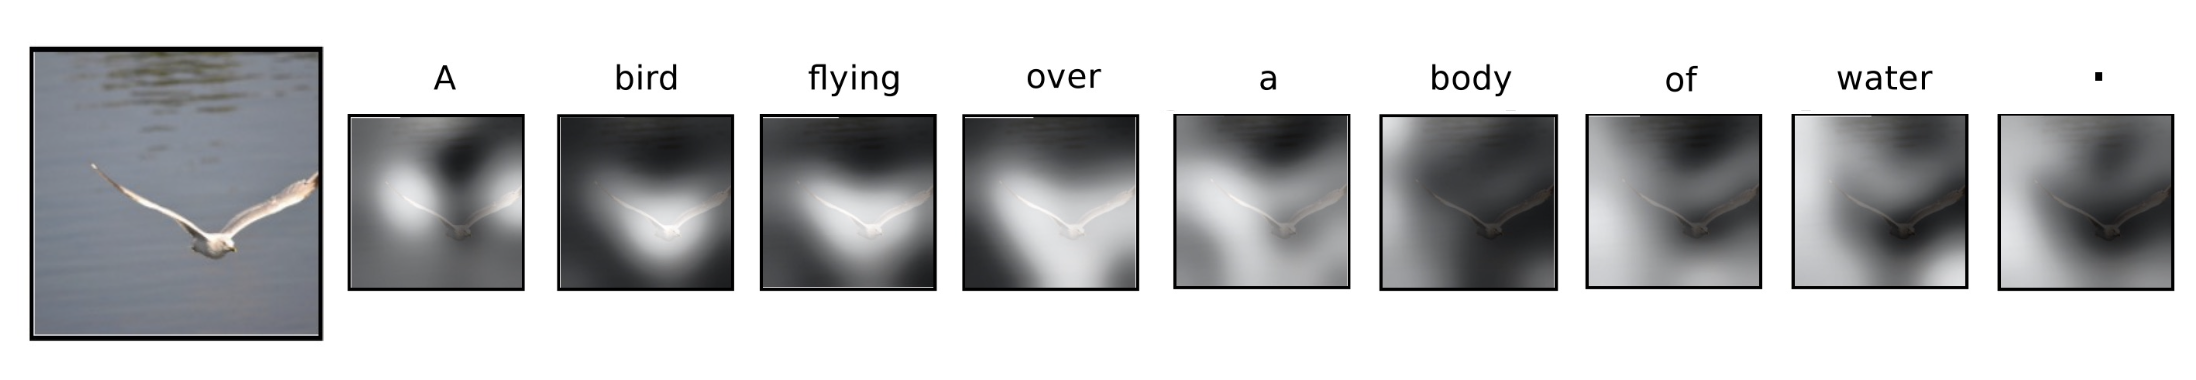
\includegraphics[width=\textwidth]{images/attention-bird.png}
    \caption{Visualizing attention over time during captioning.\protect\footnotemark}
\end{figure}
\footnotetext{Image taken from Xu et al., \say{Show, Attend, and Tell: Neural Image Caption Generation with Visual Attention}, ICML 2015}

\subsection{Attention Layer}
We saw that attention could be used in a variety of situations, for input data such as hidden states of an RNN or features grid of a CNN. The attention mechanism can be generalized into an \emph{Attention Layer}, which provides an abstraction to use attention in diverse contexts.

\subsubsection{Simple generalization}
Let's start by building an attention layer which exactly mimics the behavior described previously. In its simplest form, it uses the following inputs:
\begin{itemize}
    \item A \emph{query vector} $q$ of size $D_Q$ (the equivalent of the decoder states vectors $s_t$)
    \item A set of \emph{inputs vectors} $X$ of shape $N_X\times D_X$ (the equivalent of the encoder states vector $h_i$)
    \item A \emph{similarity function} $f_{\textnormal{acc}}:\R^{D_Q}\times\R^{D_X} \longrightarrow \R$ that can take $q$ and a certain $X_i$ as inputs and return their similarity (or alignment score)
\end{itemize}
Like we detailled previously, the computations done by the attention layer are:
\begin{itemize}
    \item The similarities $e$ of shape $N_X$, obtained by setting $e_i = f_{\textnormal{acc}}(q, X_i)$
    \item The attention weights $a=\softmax(e)$ of shape $N_X$
    \item The output vector $y = \sum_i a_i X_i$ of shape $D_X$
\end{itemize}

\subsubsection{Changing the similarity function}
While early papers on attention used a specialized function $f_{\textnormal{acc}}$ to compute similarity, it turns out to be much more simple and efficient to simply use a dot product for similarity, while keeping the same performances. Therefore, we change $X$ to be of shape $N_X\times D_Q$, and we compute the similarities with:
\begin{equation*}
    e_i = q\cdot X_i
\end{equation*}

In practice, large similarities will cause $\softmax$ to saturate and give vanishing gradients: if one coefficient is much higher than the others, the softmax distribution will peak at this element, and have an almost-zero gradient everywhere. To avoid this, we normalize $e$ by dividing it by $\sqrt{D_Q}$, giving us the \emph{scaled dot product} for similarity:
\begin{equation*}
    e_i = \frac{q\cdot X_i}{\sqrt{D_Q}}
\end{equation*}

\subsubsection{Multiple query vectors}
In previous applications of the attention layer (sequence-to-sequence, image captioning), we always used a single query vector (the decoder states). We would like to generalize this to handle multiple query vectors at a time; therefore, we replace the query vector $q$ by a set of query vectors $Q$ of size $N_Q\times D_Q$. Instead of computing the similaritie score between the query vector and each input vector, we will compute the similarities for each query vector and for each input vector:
\begin{equation*}
    E_{k,i} = \frac{Q_k\cdot X_i}{\sqrt{D_Q}}
\end{equation*}
These operations can be written and implemented using a matrix multiplication:
\begin{equation}
    E = \frac{Q\times X^\tp}{\sqrt{D_Q}}
    \label{eq:similarity-matrix}
\end{equation}

To ensure that each query vector is independent of the others, we take the $\softmax$ only over the $D_Q$ dimension of $E$:
\begin{equation*}
    A_{k,i} = \softmax_i(E_k) = \softmax_i(E, \textnormal{dim=1}) = \frac{e^{E_{k,i}}}{\sum_{i'}e^{E_{k,i'}}}
\end{equation*}
where $A$ is therefore of shape $N_Q\times N_X$.

Finally, the output vector is replaced by a set of output vectors verifying:
\begin{equation*}
    Y_k = \sum_i A_{k,i}X_i
\end{equation*}
This output matrix of shape $N_Q\times D_X$ can be written directly as:
\begin{equation}
    Y = AX 
    \label{eq:output-matrix}
\end{equation}

\subsubsection{Key-value distinction}
Note that in these computations, we are using the input vectors $X$for two different things. Firstly, we use them to compute the similarities with the query vectors $Q$ (in \autoref{eq:similarity-matrix}). Secondly, we use them to compute the output vectors $Y$ (in \autoref{eq:output-matrix}). In all generality, we can see this as two different things, and might want to use two separate sets of vectors to do so. Therefore, we often separate the input vectors into \emph{key vectors} and \emph{value vectors}.

The attention layer will still take as input a query matrix $Q$ and an input matrix $X$, but will also use a learnable \emph{key matrix} $W_K$ of shape $D_X\times D_Q$ and a learnable \emph{value matrix} $W_V$ of shape $D_X\times D_V$. These learnable matrices will be used to translate the input vectors $X$ into key vectors $K$ and value vectors $V$:
\begin{equation*}
    \begin{cases}
        K = X\times W_K\\
        V = X\times W_V
    \end{cases}
\end{equation*}
The similarities will then be computed using the key vectors:
\begin{equation*}
    E = Q\times K^\tp
\end{equation*}
and the output vectors of shape $N_Q\times D_V$ will be computed using the value vectors:
\begin{equation*}
    Y = A\times V
\end{equation*}

\begin{figure}[H]
    \centering
    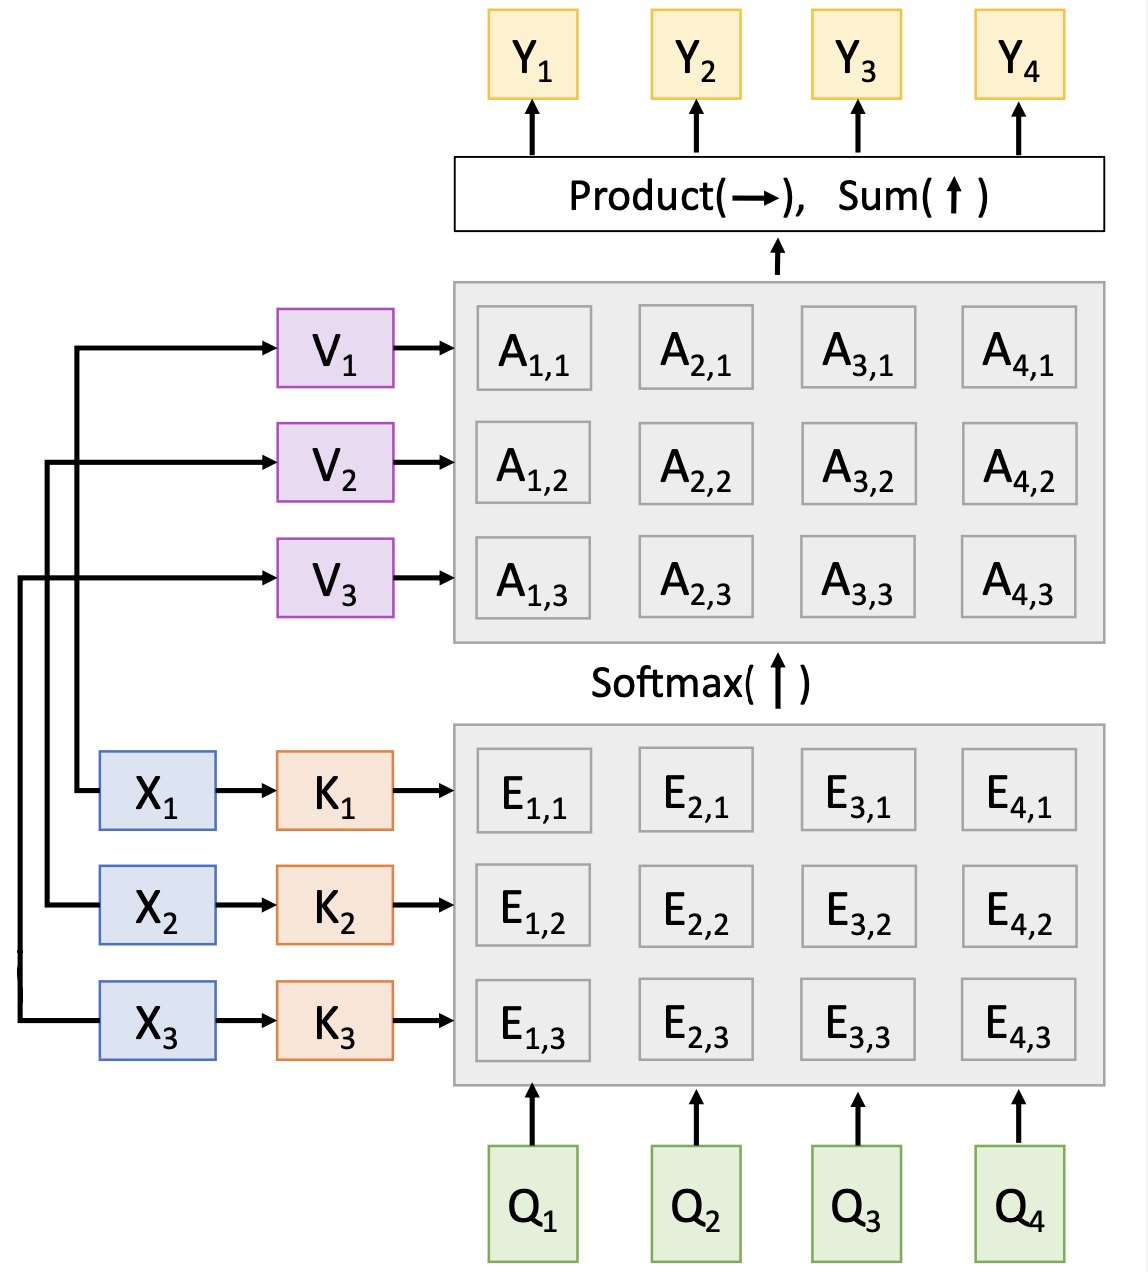
\includegraphics[width=.4\textwidth]{images/attention-layer.png}
    \caption{Schema of the attention layer making the distinction between keys and values.}
\end{figure}

\subsection{Self-Attention Layer}
\subsubsection{Principle}
We introduced a general architecture for the attention layer, which allows us to \say{search} for certain queries $Q$ into some inputs $X$. A special case of this, often used in practice, is the \emph{Self-Attention layer}: we only consider one input matrix $X$, which will be used both for inputs and queries.

Similarly to the key and value matrices, we will predict the query matrix $Q$ using the input matrix $X$. We therefore add another learnable matrix $W_Q$ of shape $D_X\times D_Q$, and we retrieve $Q$ by computing:
\begin{equation*}
    Q = X\times W_Q
\end{equation*}
Everything else works in the exact same way as the attention layer with key-value distinction.

\begin{figure}[H]
    \centering
    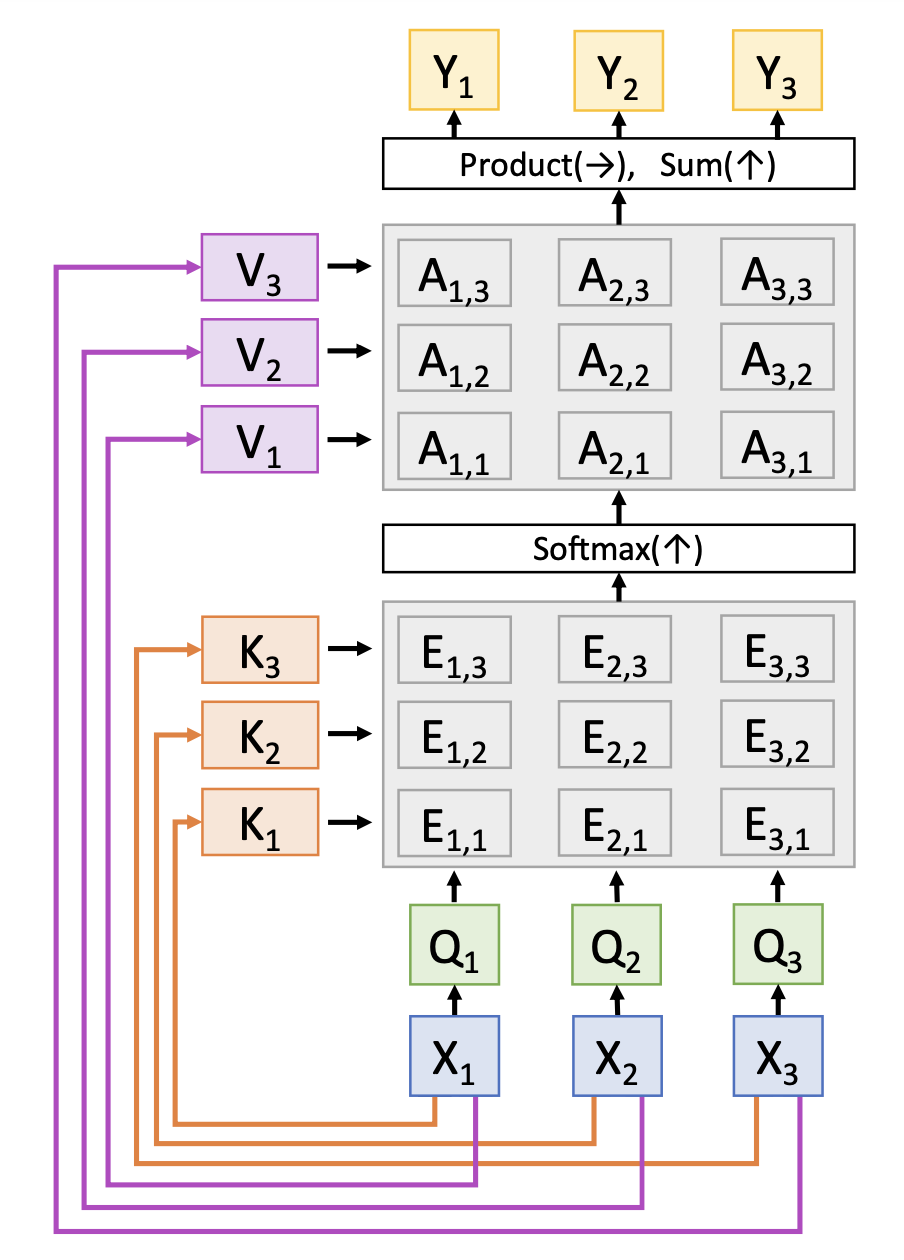
\includegraphics[width=.35\textwidth]{images/self-attention-layer.png}
    \caption{Self-attention layer.}
\end{figure}

\subsubsection{Positional encoding}
Note that permuting the input vectors will propagate the permutation up to the outputs; the self-attention layer is \emph{permutation equivariant}, which can be interpreted as the fact that it works on a set of vectors. 

This behavior might actually be unwanted, as the position of the vectors might bring more information. In order to make the self-attention processing aware of the positions, we often concatenate the input with the \emph{positional encoding} of the vectors.

To do so, we often use a learned lookup table $P$, and append at the end of the $i$-th input vector the coefficient $P(i)$. This can also be done with a fixed -- not-learned -- function.

\subsubsection{Masked Self-Attention Layer}
For certain applications, such as language modelling where we want to predict the next word, we do not want the vectors to \say{look ahead} in the sentence, but only consider the previous vectors. In an RNN, this happens already by design, because of the way that the outputs are generated.

This behavior can be manually enforced in self-attention layers. To do so, we \emph{mask} the layer, by setting some similarity scores $E_{k,i}$ to $-\infty$. This will set the corresponding attention scores $A_{k,i}$ to 0 because of the $\softmax$ formula; this way, the \say{future vectors} will not be taken into account when computing the weighted sum.

\begin{figure}[H]
    \centering
    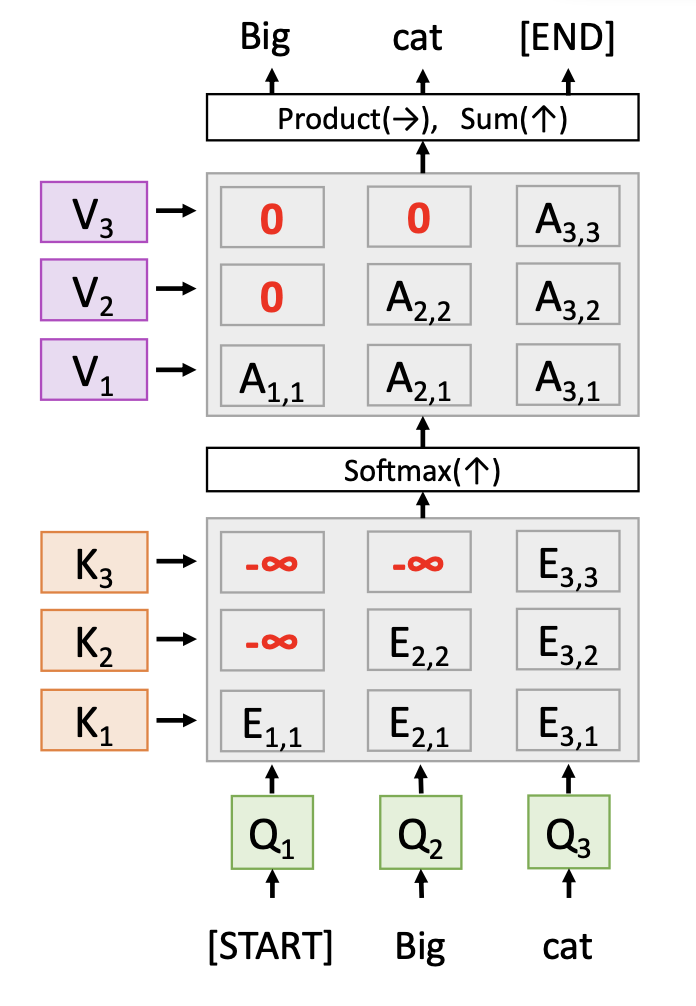
\includegraphics[width=.35\textwidth]{images/masked-attention.png}
    \caption{Masked self-attention layer.}
\end{figure}

\subsubsection{Multi-Head Self-Attention Layer}
Another variant of the attention layer is the \emph{multi-head self-attention layer}. The idea is to use $H$ \say{attention heads} in parallel, running $H$ attention layers independently. Each input vector $X_k$ is split into $H$ chunks of equal sizes; all $H$ sets of chunks are then fed into separate self-attention layers, producing $H$ sets of output chunks which are then concatenated to produce the output vectors $Y_k$. This architecture is quite common in practice.

Such layers are used with two hyperparameters: $D_Q$, the query dimension, and $H$, the number of heads.
\begin{figure}[H]
    \centering
    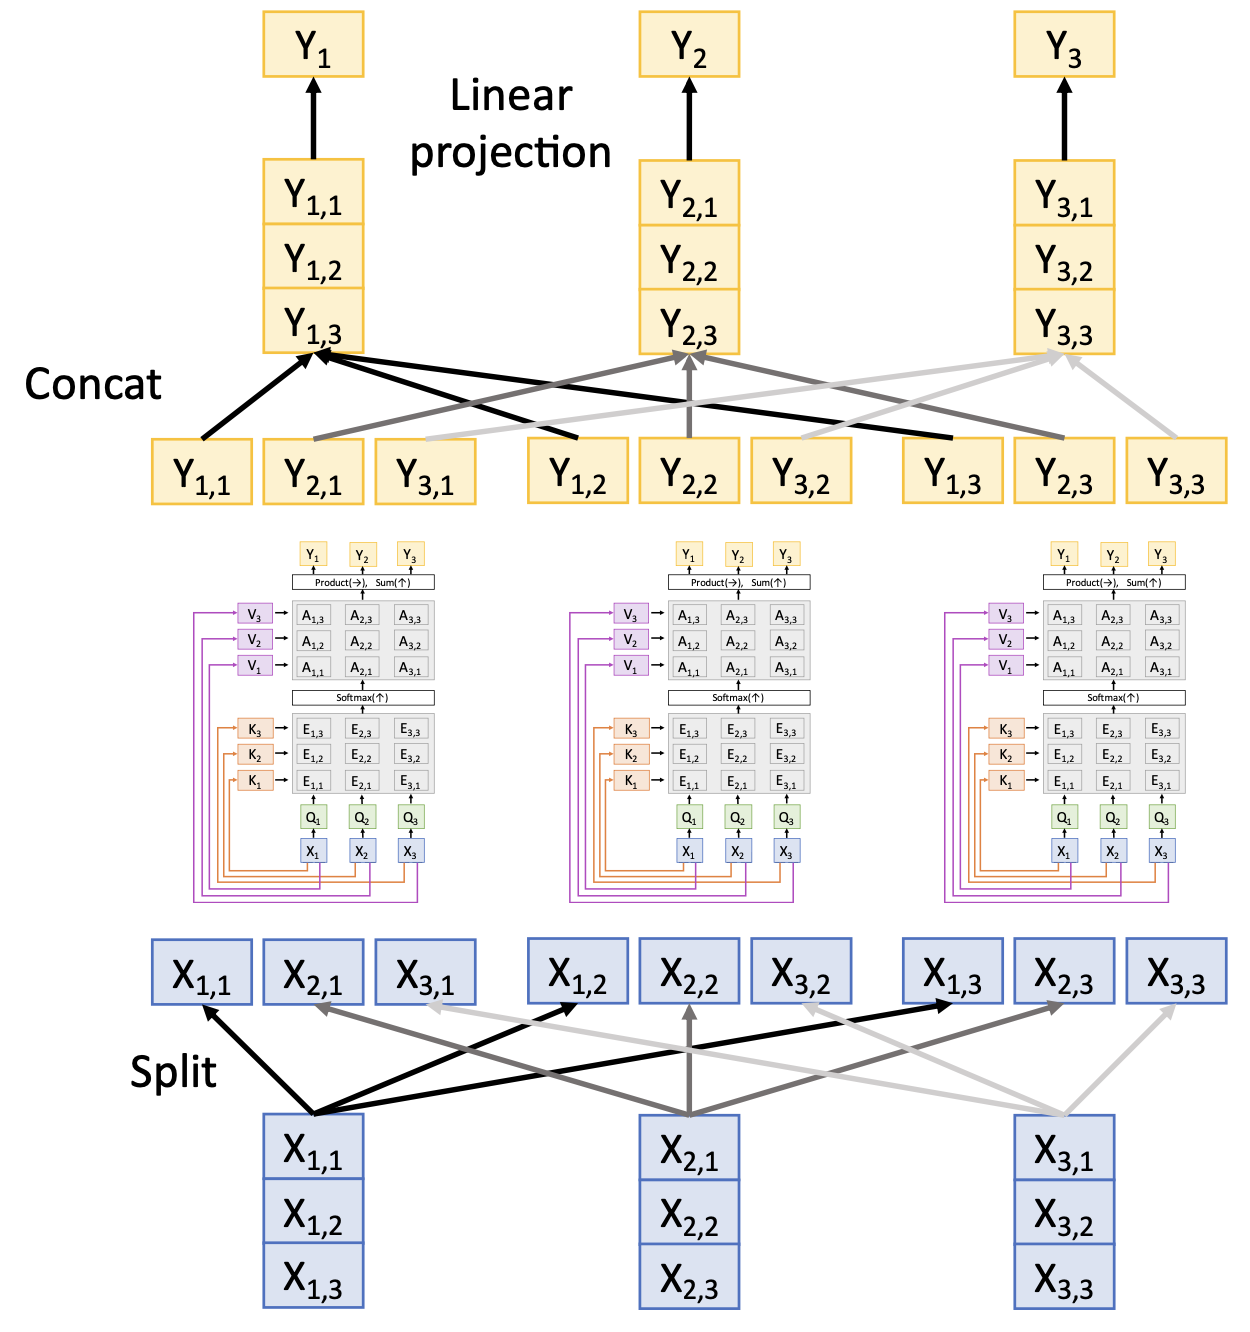
\includegraphics[width=.45\textwidth]{images/multi-head-attention.png}
    \caption{Multi-head self-attention layer.}
\end{figure}

\subsubsection{Example: CNN with Self-Attention}
\begin{figure}[H]
    \centering
    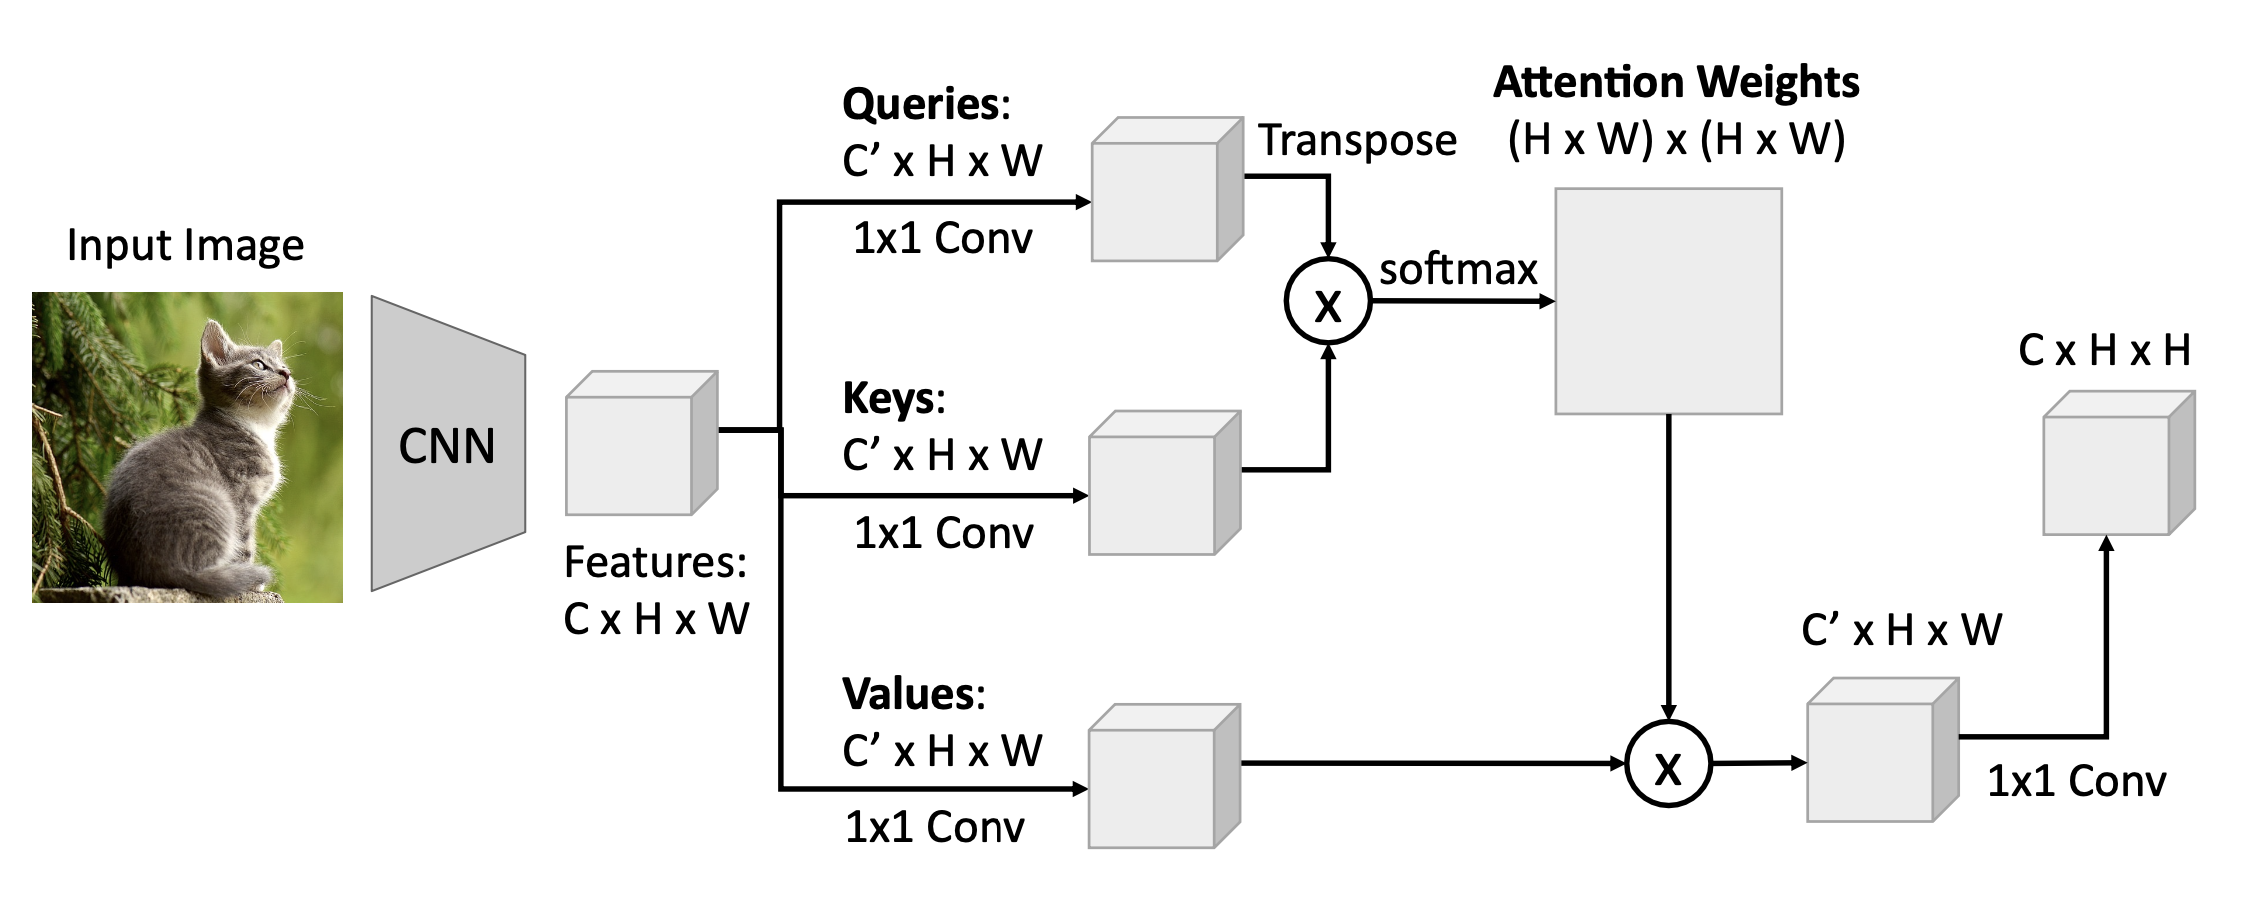
\includegraphics[width=.85\textwidth]{images/self-attention-cnn.png}
    \caption{Self-attention layer used after the output of a CNN.}
\end{figure}

\newpage